\documentclass{article}

% Revision of g1_tccml_neurips2026.tex (that file is left unchanged).
% Fig.~2 is a new equal-panel scoreboard (plot_results_equal_panels.py)
% drawn from the same numbers as the IEEE Gate~G1 table.

\PassOptionsToPackage{numbers,sort&compress}{natbib}
\usepackage{tackling_climate_workshop_style}
% Official kit footer names the workshop; this revision uses a shorter line.
\makeatletter
\renewcommand{\@noticestring}{%
  Submitted to a NeurIPS 2026 workshop.%
}
\makeatother

\usepackage[utf8]{inputenc}
\usepackage[T1]{fontenc}
\usepackage{amsmath,amssymb}
\usepackage{graphicx}
\usepackage{booktabs}
\usepackage{url}
\usepackage{microtype}
\usepackage[pdfauthor={},pdfcreator={},pdfproducer={}]{hyperref}

\title{Seasonal odds for water-energy planning: AI-ready teleconnection data and a logistic-referenced residual Transformer}

\author{%
  Dali Wang\thanks{Corresponding author.} \\
  Oak Ridge National Laboratory \\
  Oak Ridge, TN, USA \\
  \texttt{wangd@ornl.gov} \\
  \And
  Daniel M.~Ricciuto \\
  Oak Ridge National Laboratory \\
  Oak Ridge, TN, USA \\
  \AND
  Xiaoying Shi \\
  Oak Ridge National Laboratory \\
  Oak Ridge, TN, USA 
}

\begin{document}

\maketitle

\begin{abstract}
Weeks-to-years prediction of water for energy sits between weather forecasts and long-range projections: long enough that reservoir and generation decisions matter, short enough that year-to-year variability still dominates. In the Tennessee Valley Authority (TVA) region, winter wet/dry and cool/hot regimes shift hydropower inflows and thermoelectric cooling demand, so even categorical seasonal \emph{odds} would be a useful planning product for reservoir and generation operations. The problem is hard. Labelled winters are few; month-by-month anomaly regression on teleconnections collapses toward climatology; and operational seasonal systems such as CFSv2 are only a weak \emph{local} guide for categorical wet/dry outcomes. We therefore isolate a first experiment whose purpose is to test whether a documented large-scale ocean--atmosphere state can shift TVA winter odds at all, before any cascade to streamflow or energy models. All learners share one AI-ready pack of teleconnection indices and sea-surface temperature (SST) boxes. A multinomial logistic model is the skill reference. On a blocked test of 15 winters, logistic hit rate and Heidke skill for wet/dry are \(0.67\) and \(0.43\) (\(10/15\) winters), versus \(0.47\) and \(0.11\) (\(7/15\)) for October-initialized CFSv2 on the same reanalysis labels. Fully connected, LSTM, and CNN models do not match that reference; a residual temporal Transformer (logistic path plus a constrained attention residual) matches it on both tasks, with a Brier-skill gain on wet/dry rather than a higher hit rate. Skill is mainly a winter signal and fades beyond about two seasons. The result is evidence that the seasonal-odds question is tractable---not a weeks-to-years hydrology system and not an operational TVA product.
\end{abstract}

\section{Introduction}

\paragraph{A challenging but meaningful problem.}
Water for energy is decided on a weeks-to-years horizon that neither tomorrow's weather model nor a century-scale projection is built to serve.
Hydropower and thermoelectric plants in the TVA region depend on water availability, streamflow, and river temperature.
A wet versus dry winter changes reservoir inflows; a cool versus hot winter changes heating and cooling load.
Those seasonal regimes are tied to large-scale ocean--atmosphere modes: ENSO for North American winter precipitation and temperature~\citep{ropelewski1986enso,kurtzman2007enso}, and the North Atlantic Oscillation (NAO) and Arctic Oscillation (AO) for much of the eastern U.S.\ winter temperature variance~\citep{hurrell1995nao,thompson1998ao}.
If public observations and machine learning can shift the \emph{odds} of those regimes, a seasonal wet/dry outlook becomes a planning input for existing TVA reservoir and hydropower operations under year-to-year variability---valuable even though it is not yet a deployed forecast.

The same problem is scientifically hard.
The usable sample is small once winters are blocked for honest evaluation.
Pooling every calendar month as a continuous anomaly dilutes the seasonal signal, so mean-squared-error models look near climatology.
Operational seasonal products such as CFSv2~\citep{saha2014cfsv2}, a member of the North American Multi-Model Ensemble (NMME)~\citep{kirtman2014nmme}, need not be a strong \emph{local} categorical baseline for TVA wet/dry verification.
A full cascade from large-scale predictors to streamflow and energy-economy indicators cannot create skill that is absent in the index-to-seasonal-target step.

\paragraph{Purpose of this experiment.}
We therefore design a constrained first test: can autumn teleconnection indices and tropical Pacific SST, drawn from one curated pack, shift December--February (DJF) TVA wet/dry and cool/hot tercile odds?
If that signal cannot be recovered with a transparent logistic model, later spatial, land-runoff, or energy models are unlikely to invent it.
The experiment is an early step in a U.S.\ Department of Energy Genesis Mission project on water for energy; it is evidence-oriented on public data, not an operational TVA system.

\begin{figure}[t]
\centering
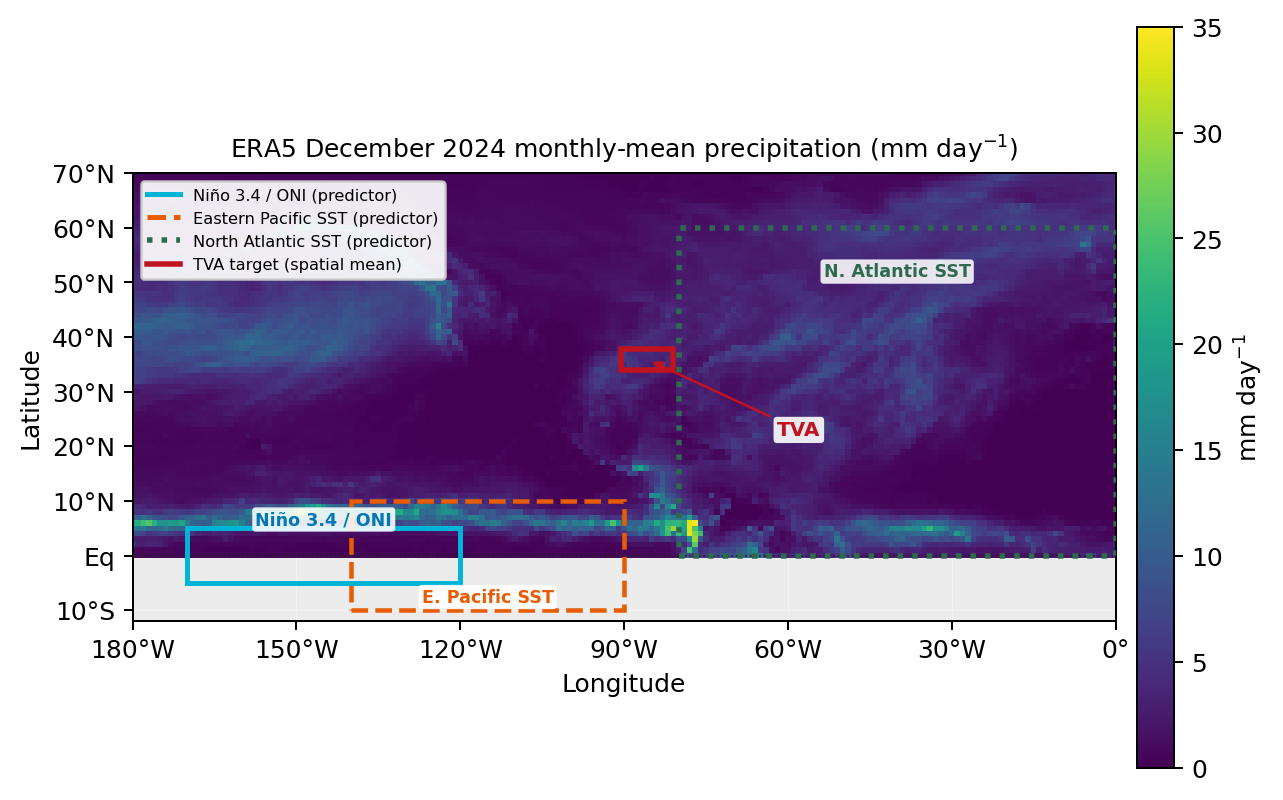
\includegraphics[width=0.74\linewidth]{figures/domain_indices_sst_tva.png}
\caption{ERA5 December 2024 monthly-mean precipitation (mm\,day$^{-1}$) over the daily \(1^{\circ}\) analysis window, with the index and SST boxes used in this paper.
Cyan: Ni\~{n}o~3.4 / ONI; dashed orange: eastern Pacific SST; dotted green: North Atlantic SST; red: TVA spatial-mean target.
NAO and AO are atmospheric indices, not additional SST boxes.
The southern half of Ni\~{n}o~3.4 lies south of the ERA5 cutoff at the equator (grey); index and SST-box time series still use the full conventional box.}
\label{fig:domain}
\end{figure}

\paragraph{How, and what we find.}
Figure~\ref{fig:domain} shows the geography: teleconnection indices and three OISST boxes as predictors; a TVA ERA5 spatial mean as the target, not map pixels~\citep{cpc-oni,barnston1997nino34,huang2021oisst,hersbach2020era5}.
All models see the same inputs.
Logistic regression on September--November (SON) means is the skill reference; CFSv2 is operational context on the same ERA5 labels, not the bar a learning model must beat; a residual Transformer may only refine logistic.
On 15 blocked test winters, logistic already exceeds climatology and this local CFSv2 comparison for wet/dry (\(10/15\) versus \(7/15\) hits).

\section{Related work}

Teleconnection diagnostics have long linked tropical Pacific SST and North Atlantic pressure patterns to U.S.\ winter precipitation and temperature~\citep{ropelewski1986enso,kurtzman2007enso,hurrell1995nao,thompson1998ao}. Operational dynamical seasonal prediction---CFSv2 and NMME---provides a public benchmark~\citep{saha2014cfsv2,kirtman2014nmme,barnston2012cfsv2}, but global ENSO skill does not automatically transfer to categorical wet/dry verification on a regional energy box. Machine learning has been applied to ENSO prediction, including deep networks for multi-year ENSO~\citep{ham2019enso}. We instead score TVA winter \emph{odds} with a logistic reference so a Transformer is accepted only if it matches or improves that reference on the same curated inputs~\citep{heidke1926,brier1950,wilks2011}. We train and score on ERA5 TVA means~\citep{hersbach2020era5} and treat Daymet~\citep{thornton2021daymet} as a later dual-truth path, not this paper's target.

\section{Data}

Every model in this paper---logistic, fully connected (FC) network, LSTM, CNN, residual Transformer---and the CFSv2 categorical comparison use the same public streams: monthly teleconnection indices, including the Oceanic Ni\~{n}o Index (ONI) and Ni\~{n}o~3.4~\citep{cpc-oni,barnston1997nino34}; SST box anomalies from NOAA OISST~\citep{huang2021oisst}; and TVA-mean ERA5 anomalies of near-surface air temperature, precipitation, and mean sea-level pressure~\citep{hersbach2020era5}. These streams are issued as a monthly labelled pack: one sample per forecast issue month (\(N{=}486\) months, August 1982--January 2023) with a 12-month lookback. The experiments below do not train a second dataset; they aggregate the same series into seasonal means or terciles.

The predictand is ERA5-based, not Daymet. Daily \(1^{\circ}\) fields over the precipitation window of Fig.~\ref{fig:domain} are averaged over the TVA box, converted to monthly anomalies, then to DJF terciles (below-normal, near-normal, above-normal) with edges estimated on training winters only. Logistic regression uses SON \emph{means} of the index/SST series; sequence models use the last \(L{=}12\) months of the same series. Reserved dataset DOIs and code URLs appear in the camera-ready data statement.

\section{Methods}

\paragraph{Tasks.}
\emph{Winter wet/dry} (primary): SON ONI and Ni\~{n}o~3.4 box anomaly predict the DJF TVA precipitation tercile (dry / near / wet). \emph{Winter cool/hot}: SON NAO and AO predict the DJF near-surface temperature tercile (cool / near / hot).

\paragraph{Split.}
Train on DJF years \(\le 2007\) (\(n{=}25\)); test on \(\ge 2009\) (\(n{=}15\)); hold out 2008. Neural models use a five-seed soft-vote ensemble on test.

\paragraph{Scores.}
Hit rate is the fraction of test winters assigned the correct tercile (chance \(\approx 1/3\)). Heidke skill measures categorical skill beyond chance (\(0\) \(\approx\) chance)~\citep{heidke1926,wilks2011}. Brier skill score (BSS) is relative to climatological class frequencies~\citep{brier1950,wilks2011}; BSS \(>0\) improves on climatology as a probability forecast. These scores match a planner-facing \emph{odds} product rather than pixel RMSE. We say a model \emph{matches the logistic reference} when hit, Heidke, and BSS are all at least as large as logistic on that task.

\paragraph{Models.}
Multinomial logistic regression on SON means; an FC network on SON means; LSTM and CNN on \(L{=}12\) monthly sequences; and a residual temporal Transformer~\citep{vaswani2017attention}
\begin{equation}
\mathrm{logits}=\mathrm{logistic}(\mathrm{SON\ mean})+\mathrm{softplus}(\alpha)\,\mathrm{Transformer}(L{=}12).
\end{equation}
With \(\sim\)25 training winters, a pure sequence model must rediscover the SON-mean teleconnection from scratch and, in our trials, failed the wet/dry task. The residual form keeps the logistic path (warm-started on SON means) and lets attention learn only a constrained correction.

\section{Results}

Figure~\ref{fig:results} reports the blocked test (exact numbers in Appendix Table~\ref{tab:results}).
Panel~(a) is \emph{local operational context} on wet/dry, not a claim that a deep network outplays CFSv2.
October-initialized CFSv2 ensemble-mean precipitation is mapped to the TVA box and scored as DJF terciles against the \textbf{same ERA5 wet/dry labels}.
It exceeds the majority-class null (hit \(0.47\) versus \(0.33\)) but remains weakly skillful categorically.
Logistic regression on two autumn means is stronger (hit \(0.67\), Heidke \(0.43\)): a \(10/15\) versus \(7/15\) difference on this pilot test.
CFSv2 is therefore context, not the reference a learning model must beat.

\begin{figure}[t]
\centering
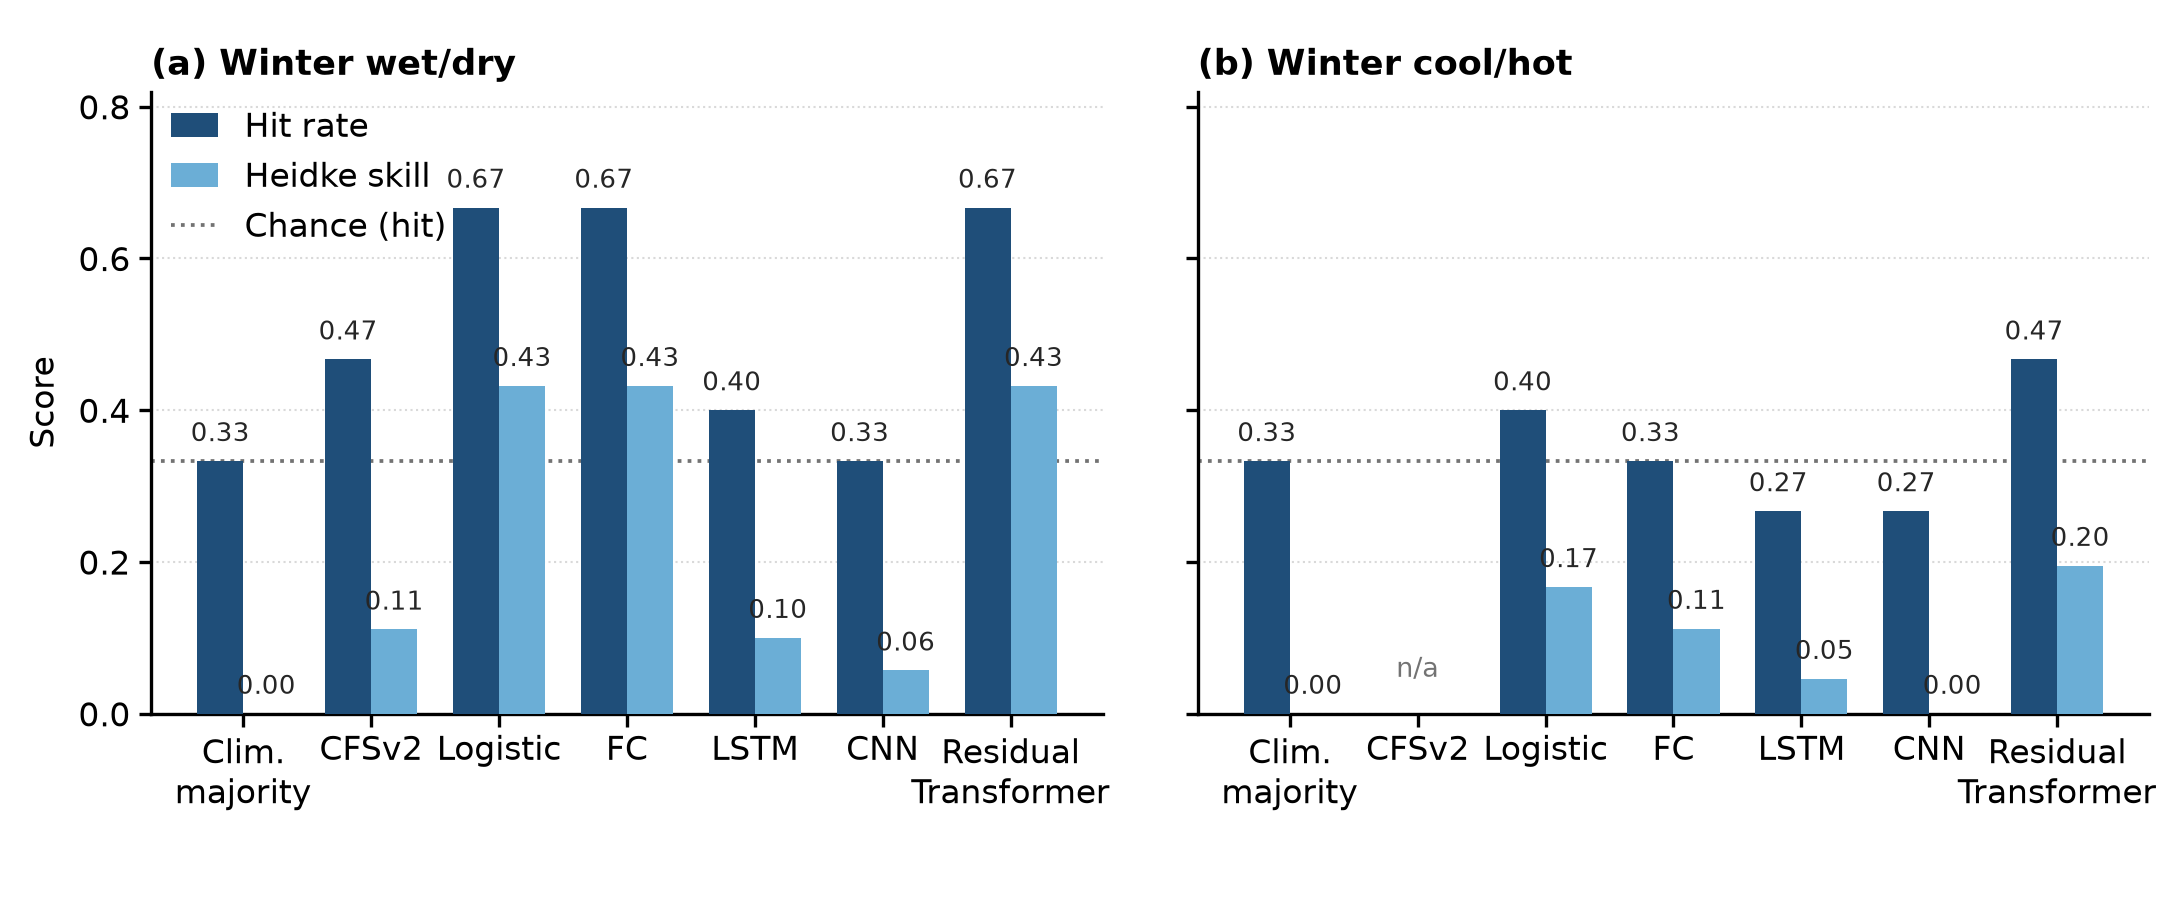
\includegraphics[width=\linewidth]{figures/results_equal_panels.png}
\caption{Blocked test (\(n{=}15\)) on identical AI-ready predictors; both panels use the same axes, bar width, and model order.
(a)~Winter wet/dry, including October-initialized CFSv2 scored on the same ERA5 labels (local context, not a full CFSv2 verification).
(b)~Winter cool/hot; CFSv2 was not scored on this task.
Dotted line: chance hit (\(1/3\)). Logistic is the skill reference; the residual Transformer matches it on hit and Heidke for wet/dry.}
\label{fig:results}
\end{figure}

Panel~(b) compares architectures on those same predictors.
FC clones logistic wet/dry hit and Heidke but not BSS.
LSTM and CNN fail the wet/dry task at this sample size.
Only the residual Transformer matches logistic on all three metrics for both tasks; on wet/dry it is tied on hit and Heidke and improves BSS (\(0.091\) to \(0.140\)).
``Strongest'' means strongest among this closed comparison, and the winning model still contains a logistic branch.
Cool/hot remains modest (logistic hit \(0.40\); Transformer \(0.47\), one extra winter).

\section{Discussion and limitations}

Two extra checks bound the claim. Using the same winter-style indices on other meteorological seasons, spring and summer do not pass; autumn wet/dry is only a weak exploratory check (hit \(0.40\), negative Heidke; Appendix~\ref{app:bounds}). Lengthening lead while keeping winter wet/dry as the target, a one-season issue (SON$\rightarrow$DJF) reproduces the main result; two seasons (JJA$\rightarrow$DJF) is a weak check (hit \(0.40\), BSS \(+0.024\)); three seasons (MAM$\rightarrow$DJF) fails. A residual Transformer does not match logistic at the two-season lead. Useful index horizon is therefore about one to two seasons for winter wet/dry, not three seasons and not all calendars.

The test set contains only 15 winters, so scores are a pilot demonstration rather than an operational skill claim; we do not report interval estimates. Cool/hot skill is modest; the water-energy narrative is primarily wet/dry. The residual Transformer is not trained from a blank slate. CFSv2 is evaluated here for TVA-box categorical wet/dry odds, not as a global seasonal verification package~\citep{barnston2012cfsv2}. This work does not yet forecast streamflow, river temperature, or energy-economy outcomes; those later steps should reuse the same odds language once daily or land targets exist.

\section{Conclusion}

Weeks-to-years water-for-energy planning needs seasonal TVA information that is difficult but, on AI-ready teleconnection data, tractable as winter odds. Logistic regression already exceeds climatology and this local CFSv2 categorical comparison for wet/dry; a residual Transformer is the strongest model we compared only in the sense that it matches that logistic reference, with logistic retained as the skill floor. That is evidence for a ground-up water-energy planning step---not a weeks-to-years hydrology system, not an image downscaler, and not a deployed TVA product. Next data work is a daily or weekly pack, not further architecture search on the monthly index tensor.

\begin{ack}
This research was supported by the U.S.\ Department of Energy Genesis Mission / Water4Energy project (DE-FOA-0003612). It used resources of the Oak Ridge Leadership Computing Facility, a DOE Office of Science User Facility. This manuscript has been authored by UT-Battelle, LLC, under contract DE-AC05-00OR22725 with the U.S.\ Department of Energy. The U.S.\ government retains a nonexclusive, paid-up, irrevocable, worldwide license to publish or reproduce the published form of this manuscript, or allow others to do so, for U.S.\ government purposes. DOE will provide public access to these results in accordance with the DOE Public Access Plan (\url{http://energy.gov/downloads/doe-public-access-plan}).

\textbf{Data and code.} Observation pack (reserved DOI \url{https://doi.org/10.13139/ORNLNCCS/3398576}) and monthly labelled training pack (reserved DOI \url{https://doi.org/10.13139/ORNLNCCS/3409936}). Staging: \url{https://github.com/daliwang/water4energy_data}, \url{https://github.com/daliwang/water4energy_trainingData}. Models: \url{https://github.com/daliwang/water4energy_model}.

\textbf{Competing interests.} The authors declare no competing interests.
\end{ack}

\appendix
\section{Calendar transfer, longer leads, and numeric scoreboard}
\label{app:bounds}

Table~\ref{tab:multiseason} uses the same logistic recipe with a strict prior-season lag (train season-years \(\le 2007\), test \(\ge 2009\)). Table~\ref{tab:leads} keeps winter wet/dry and issues the forecast one, two, or three seasons ahead. Table~\ref{tab:results} lists the blocked-test numbers plotted in Fig.~\ref{fig:results}.

\begin{table}[h]
\caption{Logistic skill by meteorological season (strict prior-season predictors). A pass requires BSS$>0$ and (Heidke$>0$ or hit above the majority class). Autumn wet/dry meets this rule only weakly (negative Heidke) and is treated as exploratory in the main text.}
\label{tab:multiseason}
\centering
\setlength{\tabcolsep}{3.5pt}
\begin{tabular}{@{}llcccc@{}}
\toprule
\textbf{Season} & \textbf{Task} & \textbf{Hit} & \textbf{Heidke} & \textbf{BSS} & \textbf{Pass} \\
\midrule
DJF (winter) & wet/dry & 0.667 & 0.432 & 0.091 & yes \\
DJF (winter) & cool/hot & 0.400 & 0.167 & 0.009 & yes \\
MAM (spring) & wet/dry & 0.333 & $-0.304$ & $-0.207$ & no \\
MAM (spring) & cool/hot & 0.133 & $-0.016$ & $-0.122$ & no \\
JJA (summer) & wet/dry & 0.400 & 0.075 & $-0.011$ & no \\
JJA (summer) & cool/hot & 0.333 & 0.063 & $-0.091$ & no \\
SON (autumn) & wet/dry & 0.400 & $-0.125$ & 0.016 & yes$^{\ast}$ \\
SON (autumn) & cool/hot & 0.400 & $-0.063$ & $-0.295$ & no \\
\bottomrule
\end{tabular}\\[0.3em]
{\footnotesize $^{\ast}$Exploratory: BSS$>0$ but Heidke$<0$.}
\end{table}

\begin{table}[h]
\caption{Logistic winter wet/dry skill versus issue lead (cool/hot at two seasons shown for contrast).}
\label{tab:leads}
\centering
\setlength{\tabcolsep}{3.5pt}
\begin{tabular}{@{}lcccc@{}}
\toprule
\textbf{Issue $\rightarrow$ target} & \textbf{Hit} & \textbf{Heidke} & \textbf{BSS} & \textbf{Pass} \\
\midrule
SON$\rightarrow$DJF (one season) & 0.667 & 0.432 & 0.091 & yes \\
JJA$\rightarrow$DJF (two seasons) & 0.400 & 0.135 & 0.024 & yes \\
MAM$\rightarrow$DJF (three seasons) & 0.133 & $-0.121$ & $-0.230$ & no \\
JJA$\rightarrow$DJF cool/hot & 0.267 & $-0.071$ & $-0.084$ & no \\
\bottomrule
\end{tabular}
\end{table}

\begin{table}[h]
\caption{Blocked test scores on identical AI-ready predictors. CFSv2 is shown for wet/dry as operational context only.}
\label{tab:results}
\centering
\setlength{\tabcolsep}{3.5pt}
\begin{tabular}{@{}llcccc@{}}
\toprule
\textbf{Task} & \textbf{Model} & \textbf{Hit} & \textbf{Heidke} & \textbf{BSS} & \textbf{vs logistic} \\
\midrule
Wet/dry & CFSv2 Oct$\rightarrow$DJF & 0.467 & 0.111 & --- & below \\
Wet/dry & Logistic & 0.667 & 0.432 & 0.091 & reference \\
Wet/dry & FC & 0.667 & 0.432 & 0.051 & below (BSS) \\
Wet/dry & LSTM & 0.400 & 0.100 & $-0.016$ & fail \\
Wet/dry & CNN & 0.333 & 0.057 & $-0.038$ & fail \\
Wet/dry & Residual Transformer & 0.667 & 0.432 & \textbf{0.140} & \textbf{matches} \\
\midrule
Cool/hot & Logistic & 0.400 & 0.167 & 0.009 & reference \\
Cool/hot & FC & 0.333 & 0.112 & 0.043 & partial \\
Cool/hot & LSTM & 0.267 & 0.046 & 0.037 & partial \\
Cool/hot & CNN & 0.267 & 0.000 & 0.022 & partial \\
Cool/hot & Residual Transformer & \textbf{0.467} & \textbf{0.195} & \textbf{0.050} & \textbf{matches} \\
\bottomrule
\end{tabular}
\end{table}

{\small
\begin{thebibliography}{22}

\bibitem{hersbach2020era5}
H.~Hersbach \emph{et al.}, ``The ERA5 global reanalysis,'' \emph{Q.\ J.\ R.\ Meteorol.\ Soc.}, vol.~146, pp.~1999--2049, 2020.

\bibitem{huang2021oisst}
B.~Huang \emph{et al.}, ``Improvements of the Daily Optimum Interpolation Sea Surface Temperature (DOISST) Version 2.1,'' \emph{J.\ Climate}, vol.~34, pp.~2923--2939, 2021.

\bibitem{barnston1997nino34}
A.~G.~Barnston, M.~Chelliah, and S.~B.~Goldenberg, ``Documentation of a highly ENSO-related SST region in the equatorial Pacific,'' \emph{Bull.\ Amer.\ Meteor.\ Soc.}, vol.~78, pp.~1107--1109, 1997.

\bibitem{cpc-oni}
NOAA Climate Prediction Center, ``Oceanic Ni\~{n}o Index (ONI),''
\url{https://www.cpc.ncep.noaa.gov/data/indices/oni.ascii.txt}
(accessed Aug.\ 2026).

\bibitem{ropelewski1986enso}
C.~F.~Ropelewski and M.~S.~Halpert, ``North American precipitation and temperature patterns associated with the El Ni\~{n}o/Southern Oscillation (ENSO),'' \emph{Mon.\ Wea.\ Rev.}, vol.~114, pp.~2352--2362, 1986.

\bibitem{kurtzman2007enso}
D.~Kurtzman and B.~R.~Scanlon, ``El Ni\~{n}o--Southern Oscillation and Pacific Decadal Oscillation impacts on precipitation in the southern and central United States,'' \emph{Water Resour.\ Res.}, vol.~43, W10417, 2007.

\bibitem{hurrell1995nao}
J.~W.~Hurrell, ``Decadal trends in the North Atlantic Oscillation: Regional temperatures and precipitation,'' \emph{Science}, vol.~269, pp.~676--679, 1995.

\bibitem{thompson1998ao}
D.~W.~J.~Thompson and J.~M.~Wallace, ``The Arctic Oscillation signature in the wintertime geopotential height and temperature fields,'' \emph{Geophys.\ Res.\ Lett.}, vol.~25, pp.~1297--1300, 1998.

\bibitem{saha2014cfsv2}
S.~Saha \emph{et al.}, ``The NCEP Climate Forecast System Version 2,'' \emph{J.\ Climate}, vol.~27, pp.~2185--2208, 2014.

\bibitem{kirtman2014nmme}
B.~P.~Kirtman \emph{et al.}, ``The North American Multimodel Ensemble,'' \emph{Bull.\ Amer.\ Meteor.\ Soc.}, vol.~95, pp.~585--601, 2014.

\bibitem{barnston2012cfsv2}
A.~G.~Barnston \emph{et al.}, ``Skill of real-time seasonal ENSO model predictions during 2002--11,'' \emph{Bull.\ Amer.\ Meteor.\ Soc.}, vol.~93, pp.~631--651, 2012.

\bibitem{ham2019enso}
Y.-G.~Ham, J.-H.~Kim, and J.-J.~Luo, ``Deep learning for multi-year ENSO forecasts,'' \emph{Nature}, vol.~573, pp.~568--571, 2019.

\bibitem{heidke1926}
P.~Heidke, ``Berechnung des Erfolges und der G\"{u}te der Windst\"{a}rkevorhersagen im Sturmwarnungsdienst,'' \emph{Geogr.\ Ann.}, vol.~8, pp.~301--349, 1926.

\bibitem{brier1950}
G.~W.~Brier, ``Verification of forecasts expressed in terms of probability,'' \emph{Mon.\ Wea.\ Rev.}, vol.~78, pp.~1--3, 1950.

\bibitem{wilks2011}
D.~S.~Wilks, \emph{Statistical Methods in the Atmospheric Sciences}, 3rd~ed.\ Academic Press, 2011.

\bibitem{vaswani2017attention}
A.~Vaswani \emph{et al.}, ``Attention is all you need,'' in \emph{Proc.\ NeurIPS}, 2017.

\bibitem{thornton2021daymet}
P.~E.~Thornton \emph{et al.}, ``Gridded daily weather data for North America with comprehensive uncertainty quantification,'' \emph{Sci.\ Data}, vol.~8, 190, 2021.

\end{thebibliography}
}

\end{document}
